\documentclass[a4paper,UKenglish,cleveref, autoref, thm-restate]{lipics-v2021}
%This is a template for producing LIPIcs articles. 
%See lipics-v2021-authors-guidelines.pdf for further information.
%for A4 paper format use option "a4paper", for US-letter use option "letterpaper"
%for british hyphenation rules use option "UKenglish", for american hyphenation rules use option "USenglish"
%for section-numbered lemmas etc., use "numberwithinsect"
%for enabling cleveref support, use "cleveref"
%for enabling autoref support, use "autoref"
%for anonymousing the authors (e.g. for double-blind review), add "anonymous"
%for enabling thm-restate support, use "thm-restate"
%for enabling a two-column layout for the author/affilation part (only applicable for > 6 authors), use "authorcolumns"
%for producing a PDF according the PDF/A standard, add "pdfa"

\pdfoutput=1 %uncomment to ensure pdflatex processing (mandatatory e.g. to submit to arXiv)
\hideLIPIcs  %uncomment to remove references to LIPIcs series (logo, DOI, ...), e.g. when preparing a pre-final version to be uploaded to arXiv or another public repository

%\graphicspath{{./graphics/}}%helpful if your graphic files are in another directory

\bibliographystyle{plainurl}% the mandatory bibstyle

\title{Towards Practical First-Order Model Counting}

\author{Ananth K. Kidambi}{Indian Institute of Technology Bombay, Mumbai, India}{210051002@iitb.ac.in}{}{}
\author{Guramrit Singh}{Indian Institute of Technology Bombay, Mumbai, India}{guramrit@iitb.ac.in}{}{}
\author{Paulius Dilkas}{University of Toronto, Toronto, Canada \and Vector Institute, Toronto, Canada \and \url{https://dilkas.github.io/}}{paulius.dilkas@utoronto.ca}{https://orcid.org/0000-0001-9185-7840}{}
\author{Kuldeep S. Meel}{University of Toronto, Toronto, Canada \and \url{https://www.cs.toronto.edu/~meel/}}{meel@cs.toronto.edu}{https://orcid.org/0000-0001-9423-5270}{}

\authorrunning{A.\,K. Kidambi, G. Singh, P. Dilkas, and K.\,S. Meel}
\Copyright{Ananth K. Kidambi, Guramrit Singh, Paulius Dilkas, and Kuldeep S. Meel}

\ccsdesc{Theory of computation~Automated reasoning}
\ccsdesc{Theory of computation~Logic and verification}
\ccsdesc{Mathematics of computing~Combinatorics}

\keywords{first-order model counting, knowledge compilation, lifted inference}

\relatedversion{} %optional, e.g. full version hosted on arXiv, HAL, or other respository/website

%\supplement{}%optional, e.g. related research data, source code, ... hosted on a repository like zenodo, figshare, GitHub, ...
%\supplementdetails[linktext={opt. text shown instead of the URL}, cite=DBLP:books/mk/GrayR93, subcategory={Description, Subcategory}, swhid={Software Heritage Identifier}]{General Classification (e.g. Software, Dataset, Model, ...)}{URL to related version} %linktext, cite, and subcategory are optional

\funding{This research was funded in part by the Natural Sciences and
  Engineering Research Council of Canada (NSERC), funding reference number
  RGPIN-2024-05956, and the Digital Research Alliance of Canada
  (\texttt{\href{https://alliancecan.ca/}{alliancecan.ca}}).}

\acknowledgements{The first two authors contributed equally. Part of the
  research was conducted while all authors were at the National University of
  Singapore.}

%\nolinenumbers %uncomment to disable line numbering



%Editor-only macros:: begin (do not touch as author)%%%%%%%%%%%%%%%%%%%%%%%%%%%%%%%%%%
\EventEditors{John Q. Open and Joan R. Access}
\EventNoEds{2}
\EventLongTitle{42nd Conference on Very Important Topics (CVIT 2016)}
\EventShortTitle{CVIT 2016}
\EventAcronym{CVIT}
\EventYear{2016}
\EventDate{December 24--27, 2016}
\EventLocation{Little Whinging, United Kingdom}
\EventLogo{}
\SeriesVolume{42}
\ArticleNo{23}
%%%%%%%%%%%%%%%%%%%%%%%%%%%%%%%%%%%%%%%%%%%%%%%%%%%%%%

\usepackage[linesnumbered,ruled,vlined]{algorithm2e}
\usepackage{siunitx}
\usepackage{tikz}
\usepackage{microtype}
\usepackage[backgroundcolor=lightgray]{todonotes} % TODO: temporary
\usepackage{mathtools}

\usetikzlibrary{arrows.meta}
\usetikzlibrary{fit}
\usetikzlibrary{positioning}
\usetikzlibrary{shapes.misc}

\newcommand{\expr}{\mathtt{expr}}
\newcommand{\FO}{$\mathsf{FO}$}
\newcommand{\Cranetwo}{\textsc{Gantry}}
\newcommand{\Cranebfs}{\textsc{Gantry-BFS}}
\newcommand{\Cranegreedy}{\textsc{Gantry-Greedy}}
\newcommand{\friends}{\emph{Friends \& Smokers}}
\newcommand{\functions}{\emph{Functions}}
\newcommand{\bijections}{\emph{Bijections}}

\SetKwProg{Fn}{Function}{:}{}
\SetKwData{Cache}{Cache}

\SetKwFunction{CompileWithBaseCases}{CompileWithBaseCases}
\SetKwFunction{Compile}{{\normalfont \textsc{Crane}}}
\SetKwFunction{Propagate}{Propagate}
\SetKwFunction{FindBaseCases}{FindBaseCases}
\SetKwFunction{Simplify}{Simplify}
\SetKwFunction{Main}{Main}
\SetKwFunction{Input}{ParseCommandLineArguments}

\DeclareMathOperator{\CR}{CR}
\DeclareMathOperator{\DR}{DR}
\DeclareMathOperator{\Reff}{Ref}
\DeclareMathOperator{\Doms}{Doms}

\sisetup{group-separator = {,}}
\newtheorem{assumption}[theorem]{Assumption}

\crefalias{enumi}{type}
\crefname{type}{Type}{Types}
\creflabelformat{type}{#2\textup{#1}#3}
\crefalias{clause}{equation}
\crefname{clause}{Clause}{Clauses}
\creflabelformat{clause}{#2\textup{(#1)}#3}
\crefalias{formula}{equation}
\crefname{formula}{Sentence}{Sentence}
\creflabelformat{formula}{#2\textup{(#1)}#3}

\begin{document}

\maketitle

\begin{abstract}
  First-order model counting (FOMC) is the problem of counting the number of
  models of a sentence in first-order logic. Since lifted inference techniques
  rely on reductions to variants of FOMC, the design of scalable methods for
  FOMC has attracted attention from both theoreticians and practitioners over
  the past decade. Recently, a new approach based on first-order knowledge
  compilation was proposed. This approach, called \textsc{Crane}, instead of
  simply providing the final count, generates definitions of (possibly
  recursive) functions that can be evaluated with different arguments to compute
  the model count for any domain size. However, this approach is not fully
  automated, as it requires manual evaluation of the constructed functions. The
  primary contribution of this work is a fully automated compilation algorithm,
  called \Cranetwo{}, which transforms the function definitions into C++ code
  equipped with arbitrary-precision arithmetic. These additions allow the new
  FOMC algorithm to scale to domain sizes over \num{500000} times larger than
  the current state of the art, as demonstrated through experimental results.
\end{abstract}

\todo[inline,caption={}]{
  For the entire paper:
  \begin{itemize}
    \item 15 pages excluding references
    \item Make sure all the internal references (e.g., to examples) are still
          valid
    \item Maybe add extra references to subsections
    \item When submitting: go through the rest of formatting instructions (in
          GTD)
  \end{itemize}
}
\section{Introduction}

\todo[inline,caption={}]{
  \begin{itemize}
    \item We would like to clarify that the main contribution of this work
          consists of everything needed to complement recursive function
          definitions with the necessary base cases. This process includes
          identifying the base cases and their corresponding sentences,
          transforming them (including applying a new smoothing procedure), and
          recursively reusing Crane. C++ code generation, although relatively
          straightforward, is crucial for the usability of the algorithm.
    \item Focus more on current work
  \end{itemize}
}

% 1. What is the problem?
% 2. Why is it interesting and important?

\emph{First-order model counting} (FOMC) is the task of determining the number
of models for a sentence in first-order logic over a specified domain. The
weighted variant, WFOMC, computes the total weight of these models, linking
logical reasoning with probabilistic
frameworks~\cite{DBLP:conf/ijcai/BroeckTMDR11}. It builds upon earlier efforts
in weighted model counting for propositional
logic~\cite{DBLP:journals/ai/ChaviraD08} and broader attempts to bridge logic
and
probability~\cite{DBLP:journals/ai/Nilsson86,novak2012mathematical,vsaletic2024graded}.
WFOMC is central to \emph{lifted inference}, which enhances the efficiency of
probabilistic calculations by exploiting
symmetries~\cite{DBLP:conf/ecai/Kersting12}. Lifted inference continues to
advance, with applications extending to constraint satisfaction
problems~\cite{DBLP:journals/jair/TotisDRK23} and probabilistic answer set
programming~\cite{DBLP:journals/ijar/AzzoliniR23}. Moreover, WFOMC has proven
effective at reasoning over probabilistic
databases~\cite{DBLP:journals/debu/GribkoffSB14} and probabilistic logic
programs~\cite{DBLP:journals/ijar/RiguzziBZCL17}. FOMC algorithms have also
facilitated breakthroughs in discovering integer
sequences~\cite{DBLP:conf/ijcai/SvatosJT0K23} and developing recurrence
relations for these sequences~\cite{DBLP:conf/kr/DilkasB23}. Recently, these
algorithms have been extended to perform sampling
tasks~\cite{DBLP:journals/ai/WangPWK24}.

% 3. Why is it hard? (E.g., why do naive approaches fail?)

The complexity of FOMC is generally measured by \emph{data complexity}, with a
sentence classified as \emph{liftable} if it can be solved in polynomial time
relative to the domain size~\cite{DBLP:conf/starai/JaegerB12}. While all
sentences with up to two variables are known to be
liftable~\cite{DBLP:conf/nips/Broeck11,DBLP:conf/kr/BroeckMD14}, Beame et
al.~\cite{DBLP:conf/pods/BeameBGS15} demonstrated that liftability does not
extend to all sentences, identifying an unliftable sentence with three
variables. Recent work has further extended the liftable fragment with
additional axioms~\cite{DBLP:conf/aaai/TothK23,DBLP:journals/ai/BremenK23} and
counting quantifiers~\cite{DBLP:journals/jair/Kuzelka21}, expanding our
understanding of liftability.

% 4. Why hasn't it been solved before? (Or, what's wrong with previous proposed
% solutions? How does mine differ?)

FOMC algorithms are diverse, with approaches ranging from \emph{first-order
  knowledge compilation} (FOKC) to cell
enumeration~\cite{DBLP:conf/uai/BremenK21}, local
search~\cite{DBLP:journals/pvldb/NiuRDS11}, and Monte Carlo
sampling~\cite{DBLP:journals/cacm/GogateD16}. (See the technical appendix for a
more detailed comparison of the state-of-the-art FOMC algorithms.) Among these,
FOKC-based algorithms are particularly prominent, transforming sentences into
structured representations such as circuits or graphs. Even when multiple
algorithms are able to solve the same instance, FOKC algorithms are known to
find polynomial-time solutions, where the polynomial has a lower degree compared
to other approaches~\cite{DBLP:conf/kr/DilkasB23}. The recently developed
ability of a FOKC algorithm to formulate solutions in terms of recursive
functions~\cite{DBLP:conf/kr/DilkasB23} is also noteworthy as the only other
proposed alternative is to guess recursive
relations~\cite{DBLP:conf/ilp/BarvinekB0ZK21}. Notable examples of FOKC
algorithms include \textsc{ForcLift}~\cite{DBLP:conf/ijcai/BroeckTMDR11} and its
successor \textsc{Crane}~\cite{DBLP:conf/kr/DilkasB23}.

% 5. What are the key components of my approach and results? Also include any
% specific limitations.

The \textsc{Crane} algorithm marked a significant step forward, expanding the
range of sentences handled by FOMC algorithms. However, it had notable
limitations: it required manual evaluation of function definitions to compute
model counts and introduced recursive functions without proper base cases,
making it more complex to use. To address these shortcomings, we present
\Cranetwo{}, a fully automated FOMC algorithm that overcomes the constraints of
its predecessor. \Cranetwo{} can handle domain sizes over \num{500000} times
larger than previous algorithms and simplifies the user experience by
automatically handling base cases and compiling function definitions into
efficient C++ programs.

In \cref{sec:preliminaries}, we cover some preliminaries, and in
\cref{sec:main}, we detail all our technical contributions. Finally, in
\cref{sec:experiments}, we present our experimental results, demonstrating
\Cranetwo{}'s performance compared to other FOMC algorithms, and, in
\cref{sec:conclusion}, we conclude the paper by discussing promising avenues for
future work.

\section{Preliminaries}\label{sec:preliminaries}

We begin this section by describing some notation that we will use throughout
the paper. Then, in \cref{sec:logic,sec:fomc} respectively, we introduce the
basic terminology of first-order logic and formally define (W)FOMC\@.
\Cref{sec:crane} outlines the principles of FOKC, particularly in the context of
\textsc{Crane}. Finally, in \cref{sec:algebra}, we introduce the algebraic
terminology used to describe the output of \textsc{Crane}, i.e., functions and
equations that define them.

\paragraph*{Notation}
We use $\mathbb{N}_{0}$ to represent the set of non-negative integers. In both
algebra and logic, we write $S\sigma$ to denote the application of a
\emph{substitution} $\sigma$ to an expression $S$, where
$\sigma = [x_{1} \mapsto y_{1}, x_{2} \mapsto y_{2}, \dots, x_{n} \mapsto y_{n}]$
signifies the replacement of all instances of $x_{i}$ with $y_{i}$ for all
$i = 1, \dots, n$. Additionally, for any variable $n$ and
$a, b \in \mathbb{N}_{0}$, let $[a \le n \le b] \coloneqq \begin{cases}
  1 & \text{if $a \le n \le b$} \\
  0 & \text{otherwise}
\end{cases}$.

\subsection{First-Order Logic}\label{sec:logic}

In this section, we will review the basic concepts of first-order logic as they
are used in FOKC algorithms. We begin by introducing the format used internally
by \textsc{ForcLift} and its descendants. Afterwards, we provide a high-level
description of how an arbitrary sentence in first-order logic is transformed
into this internal format.

A \emph{term} can be either a variable or a constant. An \emph{atom} can be
either $P(t_{1}, \dots, t_{m})$ (i.e., $P(\mathbf{t})$) for some predicate $P$
and terms $t_{1}, \dots, t_{m}$ or $x=y$ for some terms $x$ and $y$. The
\emph{arity} of a predicate is the number of arguments it takes, i.e., $m$ in
the case of the predicate $P$ mentioned above. We write $P/m$ to denote a
predicate along with its arity. A \emph{literal} can be either an atom (i.e., a
\emph{positive} literal) or its negation (i.e., a \emph{negative} literal). An
atom is \emph{ground} if it contains no variables, i.e., only constants. A
\emph{clause} is of the form $\forall x_{1} \in \Delta_{1}\text{.
}\forall x_{2} \in \Delta_{2}\dots\text{ }\forall x_{n} \in \Delta_{n}\text{.
}\phi(x_{1}, x_{2}, \dots, x_{n})$, where $\phi$ is a disjunction of literals
that only contain variables $x_{1}, \dots, x_{n}$ (and any constants). We say
that a clause is a \emph{(positive) unit clause} if there is only one literal
with a predicate, and it is a positive literal. Finally, a \emph{sentence} is a
conjunction of clauses. Throughout the paper, we will use set-theoretic
notation, interpreting a sentence as a set of clauses and a clause as a set of
literals.

\begin{remark*}
  Conforming with previous work~\cite{DBLP:conf/ijcai/BroeckTMDR11}, the
  definition of a clause includes universal quantifiers for all variables
  within. While it is possible to rewrite the entire sentence with all
  quantifiers at the front~\cite{hinman2018fundamentals}, the format we describe
  has proven itself convenient to work with.
\end{remark*}

\subsection{First-Order Model Counting}\label{sec:fomc}

In this section, we will formally define FOMC and its weighted variant. Note
that, although this work focuses on FOMC, for sentences with existential
quantifiers, computing the FOMC using \Cranetwo{} requires the use of WFOMC\@.
For such sentences, preprocessing (described in \cref{sec:crane}) introduces
predicates with non-unary weights that must be accounted for to compute the
correct model count.

\begin{definition}[Structure, model]\label{def:model}
  Let $\phi$ be a sentence in \FO{}. For each predicate $P/n$ in $\phi$, let
  ${(\Delta_{i}^{P})}_{i=1}^{n}$ be a list of the corresponding domains. Let
  $\sigma$ be a map from the domains of $\phi$ to their interpretations as
  finite sets such that the sets are pairwise disjoint, and the constants in
  $\phi$ are included in the corresponding domains. A \emph{structure} of $\phi$
  is a set $M$ of ground literals defined by adding to $M$ either
  $P(\mathbf{t})$ or $\neg P(\mathbf{t})$ for every predicate $P/n$ in $\phi$
  and $n$-tuple $\mathbf{t} \in \prod_{i=1}^{n} \sigma(\Delta_{i}^{P})$. A
  structure is a \emph{model} if it makes $\phi$ valid.
\end{definition}

\begin{example}[Counting bijections]\label{example:bijections}
  Let us consider the following sentence (previously examined by Dilkas and
  Belle~\cite{DBLP:conf/kr/DilkasB23}) that defines predicate $P$ as a bijection
  between two domains $\Gamma$ and $\Delta$:
  \begin{equation}\label[formula]{eq:bijections}
    \begin{gathered}
      (\forall x \in \Gamma\text{. }\exists y \in \Delta\text{. }P(x, y))\land{}\\
      (\forall y \in \Delta\text{. }\exists x \in \Gamma\text{. }P(x, y))\land{}\\
      (\forall x \in \Gamma\text{. }\forall y, z \in \Delta\text{. }P(x, y) \land P(x, z) \Rightarrow y = z)\land{}\\
      (\forall x, z \in \Gamma\text{. }\forall y \in \Delta\text{. }P(x, y) \land P(z, y) \Rightarrow x = z).
    \end{gathered}
  \end{equation}
  Let $\sigma$ be defined as $\sigma(\Gamma) \coloneqq \{\, 1, 2\,\}$, and
  $\sigma(\Delta) \coloneqq \{\,a, b\,\}$. Then \cref{eq:bijections} has two
  models:
  \[
    \{\, P(1, a), P(2, b), \neg P(1, b), \neg P(2, a) \,\} \qquad \text{and} \qquad \{\, P(1, b), P(2, a), \neg P(1, a), \neg P(2, b) \,\}.
  \]
\end{example}

\begin{remark*}
  The distinctness of domains is important in two ways. First, in terms of
  expressiveness, a clause such as $\forall x \in \Delta\text{. }P(x, x)$ is
  valid if predicate $P$ is defined over two copies of the same domain and
  invalid otherwise. Second, having more distinct domains makes the problem more
  decomposable for the FOKC algorithm. With distinct domains, the algorithm can
  make assumptions or deductions about, e.g., the first domain of predicate $P$
  without worrying how (or if) they apply to the second domain.
\end{remark*}

\begin{definition}[WFOMC instance]\label{def:instance}
  A \emph{WFOMC instance} comprises: a sentence $\phi$ in \FO{}, two (rational)
  \emph{weights} $w^{+}(P)$ and $w^{-}(P)$ assigned to each predicate $P$ in
  $\phi$, and $\sigma$ as described in \cref{def:model}. Unless specified
  otherwise, we assume all weights to be equal to 1.
\end{definition}

\begin{definition}[WFOMC~\cite{DBLP:conf/ijcai/BroeckTMDR11}]
  Given a WFOMC instance $(\phi, w^{+}, w^{-}, \sigma)$ as in
  \cref{def:instance}, the \emph{(symmetric) weighted first-order model count}
  (WFOMC) of $\phi$ is
  \begin{equation}\label{eq:wfomc}
    \sum_{M \models \phi} \prod_{P(\mathbf{t}) \in M} w^{+}(P) \prod_{\neg P(\mathbf{t}) \in M} w^{-}(P),
  \end{equation}
  where the sum is over all models of $\phi$.
\end{definition}

\subsection{Crane and First-Order Knowledge Compilation}\label{sec:crane}

As our work builds on \textsc{Crane}, in this section we will briefly outline
the steps \textsc{Crane} goes through to compile an \FO{} sentence into a set of
function definitions. We divide the inner workings of the algorithm into two
stages: preprocessing and compilation.

\subsubsection{Preprocessing}

The goal of this stage is to transform an arbitrary \FO{} sentence into the
format described in \cref{sec:logic}, most importantly by eliminating
existential quantifiers. For example, the first conjunct of
\cref{eq:bijections}, i.e.,
\begin{equation}\label[formula]{eq:skolemizationinitial}
  \forall x \in \Gamma\text{. }\exists y \in \Delta\text{. } P(x, y)
\end{equation}
is transformed into
\begin{equation}\label[formula]{eq:skolemization}
  \begin{aligned}
    (\forall x \in \Gamma\text{. } &Z(x))\land{}\\
    (\forall x \in \Gamma\text{. } \forall y \in \Delta\text{. } &Z(x) \lor \neg P(x, y))\land{}\\
    (\forall x \in \Gamma\text{. } &S(x) \lor Z(x))\land{}\\
    (\forall x \in \Gamma\text{. } \forall y \in \Delta\text{. } &S(x) \lor \neg P(x, y)),
  \end{aligned}
\end{equation}
where $Z/1$ and $S/1$ are two new predicates with $w^{-}(S) = -1$. One can check
that the WFOMC of \cref{eq:skolemizationinitial,eq:skolemization} is the same.

\subsubsection{Compilation}\label{sec:compilation}

At this stage, the preprocessed sentence is compiled into the set $\mathcal{E}$
of equations and two auxiliary maps $\mathcal{F}$ and $\mathcal{D}$.
$\mathcal{F}$ maps function names to sentences, and $\mathcal{D}$ maps function
names and argument indices to domains. $\mathcal{E}$ can contain any number of
functions, one of which (which we will always denote by $f$) represents the
solution to the FOMC problem. To compute the FOMC for particular domain sizes,
$f$ must be evaluated with those domain sizes as arguments. $\mathcal{D}$
records this correspondence between function arguments and domains.

\begin{example}\label{example:solution}
  \textsc{Crane} compiles \cref{eq:bijections} for bijection counting into
  \begin{align*}
    \mathcal{E} &= \left\{\,\begin{aligned}f(m, n) &= \sum_{l=0}^{n} \binom{n}{l}{(-1)}^{n-l}g(l, m),\\ g(l, m) &= \sum_{k=0}^{m}[0 \le k \le 1]\binom{m}{k}g(l-1, m-k)\end{aligned}\,\right\};\\
    \mathcal{D} &= \{\, (f, 1) \mapsto \Gamma, (f, 2) \mapsto \Delta, (g, 1) \mapsto \Delta^{\top}, (g, 2) \mapsto \Gamma \,\},
  \end{align*}
  where $\Delta^{\top}$ is a newly introduced domain. (We omit the definition of
  $\mathcal{F}$ as the sentences can get quite verbose.) To compute the number
  of bijections between two sets of cardinality 3, one would evaluate $f(3, 3)$,
  however, the definition of $g$ is incomplete: $g$ is a recursive function
  presented without any base cases. $\mathcal{D}$ encodes that in $f(m, n)$, $m$
  and $n$ represent $|\Gamma|$ and $|\Delta|$, respectively. Similarly, in
  $g(l, m)$, $l$ represents $|\Delta^{\top}|$, and $m$ represents $|\Gamma|$.
\end{example}

Compilation is performed primarily by applying \emph{(compilation) rules} to
sentences. \textsc{Crane} has two modes depending on how the algorithm chooses
which compilation rule to apply to a sentence (in case several alternatives are
available). The first option is to use greedy search: there is a list of rules,
and the first applicable rule is the one that gets used, disregarding all the
others. The second option is to use a combination of greedy and
\emph{breadth-first search} (BFS). That is, each compilation rule is identified
as either greedy or non-greedy. Greedy rules are applied as soon as possible at
any stage of the compilation process. BFS is executed over all applicable
non-greedy rules, identifying the solution that can be constructed using the
smallest number of such rules.

\subsection{Algebra}\label{sec:algebra}

In this paper, we use both logical and algebraic constructs. While the rest of
\cref{sec:preliminaries} focused on the former, this section describes the
latter. We write $\expr{}$ for an arbitrary algebraic expression. In the context
of algebra, a \emph{constant} is a non-negative integer. Likewise, a
\emph{variable} can either be a parameter of a function or a variable introduced
through summation, such as $i$ in the expression $\sum_{i=1}^{n} \expr$. A
\emph{function call} is $f(x_{1}, \dots, x_{n})$ (or $f(\mathbf{x})$ for short),
where $f$ is an $n$-ary function, and each $x_{i}$ is an algebraic expression
consisting of variables and constants. A (function) \emph{signature} is function
call that contains only variables. Given two function calls $f(\mathbf{x})$ and
$f(\mathbf{y})$, we say that $f(\mathbf{y})$ \emph{matches} $f(\mathbf{x})$ if
$x_{i} = y_{i}$ whenever $x_{i}, y_{i} \in \mathbb{N}_{0}$. An \emph{equation}
is $f(\mathbf{x}) = \expr{}$, where $f(\mathbf{x})$ is a function call.

\begin{definition}[Base case]\label{def:basecase}
  Let $f(\mathbf{x})$ be a function call where each $x_{i}$ is either a constant
  or a variable. Then function call $f(\mathbf{y})$ is a \emph{base case} of
  $f(\mathbf{x})$ if $f(\mathbf{y}) = f(\mathbf{x})\sigma$, where $\sigma$ is a
  substitution that replaces one or more $x_{i}$ with a constant.
\end{definition}

\begin{example}
  In equation $f(m, n) = f(m-1, n) + nf(m-1, n-1)$, the only constant is $1$,
  and the variables are $m$ and $n$. The equation contains three function calls:
  one on the left-hand side (LHS), and two on the right-hand side (RHS). The
  function call on the LHS is a signature. Function calls such as $f(4, n)$,
  $f(m, 0)$, and $f(8, 1)$ are all considered base cases of $f(m, n)$ (only some
  of which are useful).
\end{example}

\section{Technical Contributions}\label{sec:main}

\begin{figure*}[t]
  \centering
  \begin{tikzpicture}
    \node[anchor=west] at (-1, 0) (formula) {$\phi$};
    \node[draw,rounded rectangle] at (3, 0) (compilewithbasecases) {\CompileWithBaseCases};
    \node[draw,rounded rectangle] at (9, 0) (compilation) {Compile to C++};

    \node[draw,rounded rectangle,dashed] at (9, -3) (cpp) {C++ code};
    \node[anchor=west] at (-1, -3) (sizes) {Domain sizes};
    \node at (12, -3) (count) {Answer};

    \node[draw,rounded rectangle] at (3, -2) (findbasecases) {\FindBaseCases};
    \node[draw,rounded rectangle,left = 0.1cm of findbasecases] (crane) {\Compile};
    \node[draw,rounded rectangle,right = 0.1cm of findbasecases] (propagate) {\Propagate};
    \node[draw,rounded rectangle,right = 0.1cm of propagate] (simplify) {\Simplify};

    \node[draw,fit={(compilewithbasecases) (compilation) (crane) (findbasecases) (propagate)},inner ysep=7pt,yshift=5pt] {};
    \node at (0.7, 0.5) {\Cranetwo};

    \draw[-Latex] (formula) -- (compilewithbasecases);
    \draw[-Latex] (compilewithbasecases) -- node[above] {$\mathcal{E}$} (compilation);
    \draw[-Latex] (compilation) -- (cpp);
    \draw[-Latex] (sizes) -- (cpp);
    \draw[-Latex] (cpp) -- (count);

    \draw[-Latex,dashed] (compilewithbasecases) -- node[midway,left] {uses} (crane);
    \draw[-Latex,dashed] (compilewithbasecases) -- node[midway,left] {uses} (findbasecases);
    \draw[-Latex,dashed] (compilewithbasecases) -- node[midway,left] {uses} (propagate);
    \draw[-Latex,dashed] (compilewithbasecases) -- node[midway,right] {uses} (simplify);
  \end{tikzpicture}
  \caption[]{The outline of using \Cranetwo{} to compute the model count of a
    sentence $\phi$. First, $\phi$ is compiled into a set of equations, which
    are then used to create a C++ program. This program can be executed with
    different command line arguments to calculate the model count of $\phi$ for
    different domain sizes. To accomplish this, the \CompileWithBaseCases
    procedure uses \textsc{Crane}, algebraic simplification techniques (denoted
    as \Simplify), and two other auxiliary procedures. }\label{fig:overview}
\end{figure*}

\Cref{fig:overview} provides an overview of \Cranetwo{}'s workflow. Below we
briefly describe and motivate each procedure before going into more detail in
the corresponding subsection.

\CompileWithBaseCases (see \cref{sec:completing}), the core procedure of
\Cranetwo{}, is responsible for completing the function definitions produced by
\textsc{Crane} with the necessary base cases. To do so, it may recursively call
itself (and \textsc{Crane}) on other sentences. We prove that the number of such
recursive calls is upper bounded by the number of domains in the sentences.

\cref{sec:completing} also describes the \Simplify procedure for algebraic
simplification. It is crucial for simplifying, e.g., a sum of $n$ terms, only
two of which are non-zero. More generally, the equations returned by
\textsc{Crane} often benefit from easy-to-detect algebraic simplifications such
as $0 \cdot \text{anything} = 0$ and $\text{anything}^{0} = 1$.

\FindBaseCases (described in \cref{sec:identifying}) inspects a set of equations
to identify a sufficient set of base cases for a given set of equations. We
prove that the returned set of base cases is sufficient, and the evaluation of
the resulting function definitions will never get stuck in an infinite loop.

\Cref{sec:propagating} introduces the \Propagate procedure that takes a sentence
$\phi$, a domain $\Delta$, and $n \in \mathbb{N}_{0}$. It returns $\phi$
transformed with the assumption that $|\Delta| = n$, introducing $n$ new
constants and removing all variables quantified over $\Delta$. For example, when
computing a base case such as $f(0, y)$, \Propagate will significantly simplify
$\phi$ with the assumption that the domain associated with the first parameter
of $f$ (i.e., $\mathcal{D}(f, 1)$) is empty. When run on this simplified
sentence, \CompileWithBaseCases will return the equations for the base case
$f(0, y)$.

\Cref{sec:smoothing} describes a new kind of \emph{smoothing} used to ensure
that \Propagate preserves the correct model count. Smoothing is a well-known
technique in knowledge compilation algorithms for propositional model
counting~\cite{darwiche2001tractable}. Although it has been applied to FOMC
before~\cite{DBLP:conf/ijcai/BroeckTMDR11}, our setting requires a novel
approach.

\CompileWithBaseCases, together with the other procedures outlined above, return
a set of equations that fully cover the base cases of all recursive functions.
While these equations can be interesting and valuable in their own right, the
users of FOMC algorithms typically expect a numerical answer. Thus,
\cref{sec:cpp} describes how these equations are compiled into a C++ program
that can be executed with different command-line arguments to compute the model
count for different combinations of domain sizes.

\subsection{Completing the Definitions of Functions}\label{sec:completing}

\begin{algorithm}[t]
  \caption{\protect\CompileWithBaseCases{$\phi$}}\label{alg:compilewithbasecases}
  \KwIn{sentence $\phi$}
  \KwOut{set $\mathcal{E}$ of equations}
  $(\mathcal{E}, \mathcal{F}, \mathcal{D}) \gets \Compile{$\phi$}$\;
  $\mathcal{E} \gets \Simplify{$\mathcal{E}$}$\;\label{line:second}
  \ForEach{base case $f(\mathbf{x}) \in \FindBaseCases{$\mathcal{E}$}$}{\label{line:loopy}
    $\psi \gets \mathcal{F}(f)$\;
    \lForEach{index $i$ such that $x_{i} \in \mathbb{N}_{0}$}{$\psi \gets \Propagate{$\psi$, $\mathcal{D}(f, i)$, $x_i$}$}\label{line:propagate}
    $\mathcal{E} \gets \mathcal{E} \cup \CompileWithBaseCases{$\psi$}$\;\label{line:final}
  }
\end{algorithm}

\Cref{alg:compilewithbasecases} presents our overall approach for compiling a
sentence into equations that include the necessary base cases. To begin, we use
\textsc{Crane} to compile the sentence into the three components: $\mathcal{E}$,
$\mathcal{F}$, and $\mathcal{D}$ (as described in \cref{sec:compilation}). After
some algebraic simplifications (described below), $\mathcal{E}$ is passed to the
\FindBaseCases procedure (see \cref{sec:identifying}). For each base case
$f(\mathbf{x})$, we retrieve the sentence $\mathcal{F}(f)$ associated with the
function name $f$ and simplify it using the \Propagate procedure (explained in
detail in \cref{sec:propagating}). We do this by iterating over all indices of
$\mathbf{x}$, where $x_{i}$ is a constant, and using \Propagate to simplify
$\psi$ by assuming that domain $\mathcal{D}(f, i)$ has size $x_{i}$. Finally, on
\autoref{line:final}, \CompileWithBaseCases recurses on these simplified
sentences and adds the resulting base case equations to $\mathcal{E}$.

\paragraph*{Simplify}
The main responsibility of the \Simplify procedure is to handle the algebraic
pattern $\sum_{m=0}^{n}[a \le m \le b] f(m)$. Here: $n$ is a variable,
$a, b \in \mathbb{N}_{0}$ are constants, and $f$ is an expression that may
depend on $m$. \Simplify transforms this pattern into
$f(a) + f(a+1) + \cdots + f(\min\{\, n, b \,\})$.

\begin{example}\label{example:bijectionstwo}
  Let us return to the bijection-counting problem from \cref{example:bijections}
  and its initial solution described in \cref{example:solution}. \Simplify
  transforms $g(l, m) = \sum_{k=0}^{m}[0 \le k \le 1]\binom{m}{k}g(l-1, m-k)$
  into $g(l, m) = g(l-1, m) + mg(l-1, m-1)$. Then \FindBaseCases identifies two
  base cases: $g(0, m)$ and $g(l, 0)$. In both cases, \CompileWithBaseCases
  recurses on the sentence $\mathcal{F}(g)$ simplified by assuming that one of
  the domains is empty. In the first case, we recurse on the sentence
  $\forall x \in \Gamma\text{. }S(x) \lor \neg S(x)$, where $S$ is a predicate
  introduced by preprocessing with weights $w^{+}(S) = 1$ and $w^{-}(S) = -1$.
  Hence, we obtain the base case $g(0, m) = 0^{m}$. In the case of $g(l, 0)$,
  \Propagate{$\psi$, $\Gamma$, $0$} returns an empty sentence, resulting in
  $g(l, 0) = 1$. While these base cases overlap when $l = m = 0$, they remain
  consistent since $0^{0} = 1$.
\end{example}

% Generally, let $\phi$ be a sentence with two domains $\Gamma$ and $\Delta$,
% and let $n, m \in \mathbb{N}_{0}$. Then the FOMC of \Propagate{$\phi$,
% $\Delta$, $n$} assuming $|\Gamma| = m$ is the same as the FOMC of
% \Propagate{$\phi$, $\Gamma$, $m$} assuming $|\Delta| = n$.

% Although \CompileWithBaseCases starts with a call to \textsc{Crane}, the
% proposed algorithm is not just a post-processing step for FOKC because
% \cref{alg:compilewithbasecases} is recursive and can issue more calls to
% \textsc{Crane} on various derived sentences.

We end this section by proving that \CompileWithBaseCases terminates since each
recursive call on \autoref{line:final} reduces the number of domains in the
sentence.

\begin{theorem}
  Given any \FO{} sentence $\phi$, \CompileWithBaseCases{$\phi$} terminates.
\end{theorem}

\todo[inline]{Reformulate the theorem above into an upper bound (as I informally
  mention earlier in the text)}

To prove the theorem, we rely on two observations about the algorithms presented
in \cref{sec:identifying,sec:propagating}.

\begin{observation}\label{observation1}
  Each base case returned by \FindBaseCases has at least one constant (in line
  with \cref{def:basecase}).
\end{observation}

\begin{observation}\label{observation2}
  For any sentence $\phi$, domain $\Delta$, and $n \in \mathbb{N}_{0}$,
  \Propagate{$\phi$, $\Delta$, $n$} returns a sentence with no variables
  quantified over $\Delta$.
\end{observation}

\begin{proof}
  We proceed by induction on the number of domains that variables in $\phi$ are
  quantified over. If there are no domains, then $\phi$ is essentially a
  propositional formula, and \textsc{Crane} compiles it into an equation of the
  form $f = \expr$ with no `function calls'. Suppose that \CompileWithBaseCases
  terminates for all sentences with at most $n \in \mathbb{N}_{0}$ domains. Let
  $\phi$ be a sentence with $n+1$ domains. By \cref{observation1}, each base
  case on \autoref{line:loopy} of \cref{alg:compilewithbasecases} has at least
  one constant. Therefore, by \cref{observation2}, after
  \autoref{line:propagate}, sentence $\psi$ has at most $n$ domains. Thus,
  \autoref{line:final} terminates by the inductive hypothesis, completing the
  proof that \CompileWithBaseCases terminates for an arbitrary sentence with
  $n+1$ domains.
\end{proof}

\subsection{Identifying a Sufficient Set of Base Cases}\label{sec:identifying}

\begin{algorithm}[t]
  \caption{\protect\FindBaseCases{$\mathcal{E}$}}\label{alg:findbasecases}
  \KwIn{set $\mathcal{E}$ of equations}
  \KwOut{set $\mathcal{B}$ of base cases}

  $\mathcal{B} \gets \emptyset$\;
  \ForEach{function call $f(\mathbf{y})$ on the RHS of an equation in $\mathcal{E}$}{
    $\mathbf{x} \gets \text{the parameters of $f$ in its definition}$\;
    \ForEach{$y_{i} \in \mathbf{y}$} {
      \lIf{$y_{i} \in \mathbb{N}_{0}$}{$\mathcal{B} \gets \mathcal{B} \cup \{\, f(\mathbf{x})[x_{i} \mapsto y_{i}] \,\}$}
      \ElseIf{$y_{i} = x_{i} - c_{i}$ for some $c_{i} \in \mathbb{N}_{0}$}{
        \lFor{$j \gets 0$ \KwTo $c_{i} - 1$}{$\mathcal{B} \gets \mathcal{B} \cup \{\, f(\mathbf{x})[x_{i} \mapsto j] \,\}$}
      }
    }
  }
\end{algorithm}
% (later, let's not bother yet): replace x_i-c_i on Line 7 of Algorithm 2 with a
% generalisation of x_i that can be an arbitrary summation/subtraction of domain
% sizes (propagating this change to the rest of the paper, particularly
% Assumption 1, the proof of Lemma 1)

\Cref{alg:findbasecases} summarises the implementation of \FindBaseCases. It
considers two types of arguments when a function $f$ calls itself recursively:
constants and arguments of the form $x_{i} - c_{i}$. Here, $c_{i}$ is a
constant, and $x_{i}$ is the $i$-th argument of the signature of $f$. When the
argument is a constant $c_{i}$, a base case with $c_{i}$ is added. In the second
case, a base case is added for each constant from $0$ up to (but not including)
$c_{i}$.

\begin{example}
  Consider the recursive function $g$ from \cref{example:solution}.
  \FindBaseCases iterates over two function calls: $g(l-1, m)$ and
  $g(l-1, m-1)$. The former produces the base case $g(0, m)$, while the latter
  produces both $g(0, m)$ and $g(l, 0)$.
\end{example}

It can be shown that the base cases identified by \FindBaseCases are sufficient
for the algorithm to terminate.\footnote{Note that characterising the
  fine-grained complexity of the solutions found by \Cranetwo{} or other FOMC
  algorithms is an emerging area of research. These questions have been
  partially addressed in previous
  work~\cite{DBLP:conf/kr/DilkasB23,DBLP:conf/kr/TothK24}
  and are orthogonal to the goals of this section.} For the remainder of this
section, let $\mathcal{E}$ denote the equations returned by
\CompileWithBaseCases.

\begin{theorem}\label{thm:halting}
  Let $f$ be an $n$-ary function in $\mathcal{E}$ and
  $\mathbf{x} \in \mathbb{N}_{0}^{n}$. Then the evaluation of $f(\mathbf{x})$
  terminates.
\end{theorem}

We prove \cref{thm:halting} using double induction. First, we apply induction to
the number of functions in $\mathcal{E}$. Then, we use induction on the arity of
the `last' function in $\mathcal{E}$ according to some topological ordering. We
begin with a few observations that stem from
previous~\cite{DBLP:conf/kr/DilkasB23,DBLP:conf/ijcai/BroeckTMDR11} and this
work.

\begin{observation}\label{assumption1}
  For each function $f$, there is precisely one equation $e \in \mathcal{E}$
  with $f(\mathbf{x})$ on the LHS where all $x_{i}$'s are variables (i.e., $e$
  is not a base case). We refer to $e$ as the \emph{definition} of $f$.
\end{observation}

\begin{observation}\label{assumption2}
  There is a \emph{topological ordering} of all functions ${(f_{i})}_{i}$ in
  $\mathcal{E}$ such that equations in $\mathcal{E}$ with $f_{i}$ on the LHS do
  not contain function calls to $f_{j}$ with $j > i$. This condition prevents
  mutual recursion and other cyclic scenarios.
\end{observation}

\begin{observation}\label{assumption3}
  For each equation $(f(\mathbf{x}) = \expr) \in \mathcal{E}$, the evaluation
  of $\expr$ terminates when provided with the values of all relevant function
  calls.
\end{observation}

\begin{corollary}\label{fact}
  If $f$ is a non-recursive function with no function calls on the RHS of its
  definition, then the evaluation of any function call $f(\mathbf{x})$
  terminates.
\end{corollary}

\begin{observation}\label{fact2}
  For each equation $(f(\mathbf{x}) = \expr{}) \in \mathcal{E}$, if $\mathbf{x}$
  contains only constants, then $\expr{}$ cannot include any function calls to
  $f$.
\end{observation}

Additionally, we introduce an assumption about the structure of recursion.

\begin{assumption}\label{assumption4}
  For each equation $(f(\mathbf{x}) = \expr) \in \mathcal{E}$, every recursive
  function call $f(\mathbf{y}) \in \expr$ satisfies the following:
  \begin{itemize}
    \item Each $y_{i}$ is either $x_{i} - c_{i}$ or $c_{i}$ for some constant
          $c_{i}$.
    \item There exists $i$ such that $y_{i} = x_{i} - c_{i}$ for some
          $c_{i} > 0$.
  \end{itemize}
\end{assumption}

Finally, we assume a particular order of evaluation for function calls using the
equations in $\mathcal{E}$. Specifically, we assume that base cases are
considered before the recursive definition. The exact order in which base cases
are considered is immaterial.

\begin{assumption}
  When multiple equations in $\mathcal{E}$ match a function call
  $f(\mathbf{x})$, preference is given to an equation with the most constants on
  its LHS.
\end{assumption}

With the observations and assumptions mentioned above, we are ready to prove
\cref{thm:halting}. For readability, we divide the proof into several lemmas of
increasing generality.

\begin{lemma}\label{lemma:oneunary}
  Assume that $\mathcal{E}$ consists of just \emph{one unary} function $f$. Then
  the evaluation of a function call $f(x)$ terminates for any
  $x \in \mathbb{N}_{0}$.
\end{lemma}
\begin{proof}
  If $f(x)$ is captured by a base case, then its evaluation terminates by
  \cref{fact,fact2}. If $f$ is not recursive, the evaluation of
  $f(x)$ terminates by \cref{fact}.

  Otherwise, let $f(y)$ be an arbitrary function call on the RHS of the
  definition of $f(x)$. If $y$ is a constant, then there is a base case for
  $f(y)$. Otherwise, let $y = x - c$ for some $c > 0$. Then there exists
  $k \in \mathbb{N}_{0}$ such that $0 \le x - kc \le c-1$. So, after $k$
  iterations, the sequence of function calls $f(x), f(x-c), f(x-2c),\dots$ will
  be captured by the base case $f(x \mod c)$.
\end{proof}

\begin{lemma}\label{lemma:onefunction}
  Generalising \cref{lemma:oneunary}, let $\mathcal{E}$ be a set of equations
  for \emph{one} $n$-ary function $f$ for some $n \ge 1$. Then the evaluation of
  $f(\mathbf{x})$ terminates for any $\mathbf{x} \in \mathbb{N}_{0}^{n}$.
\end{lemma}
\begin{proof}
  If $f$ is non-recursive, the evaluation of $f(\mathbf{x})$ terminates by
  previous arguments. We proceed by induction on $n$, with the base case of
  $n=1$ handled by \cref{lemma:oneunary}. Assume that $n > 1$. Any base case of
  $f$ can be seen as a function of arity $n-1$, since one of the parameters is
  fixed. Thus, the evaluation of any base case terminates by the inductive
  hypothesis. It remains to show that the evaluation of the recursive equation
  for $f$ terminates, but that follows from \cref{assumption3}.
\end{proof}

\begin{proof}[Proof of \cref{thm:halting}]
  We proceed by induction on the number of functions $n$. The base case of $n=1$
  is handled by \cref{lemma:onefunction}. Let ${(f_{i})}_{i=1}^{n}$ be some
  topological ordering of these $n > 1$ functions. If $f = f_{j}$ for $j < n$,
  then the evaluation of $f(\mathbf{x})$ terminates by the inductive hypothesis
  since $f_{j}$ cannot call $f_{n}$ by \cref{assumption2}. Using the inductive
  hypothesis that all function calls to $f_{j}$ (with $j < n$) terminate, the
  proof proceeds similarly to the Proof of \cref{lemma:onefunction}.
\end{proof}

\subsection{Propagating Domain Size Assumptions}\label{sec:propagating}

\begin{algorithm}[t]
  \caption{\protect\Propagate{$\phi$, $\Delta$, $n$}}\label{alg:propagate}
  \KwIn{sentence $\phi$, domain $\Delta$, $n \in \mathbb{N}_{0}$}
  \KwOut{sentence $\phi'$}
  $\phi' \gets \emptyset$\;
  \uIf{$n = 0$}{
    \ForEach{clause $C \in \phi$}{
      \lIf{$\Delta \not\in \Doms(C)$}{$\phi' \gets \phi' \cup \{\, C \,\}$}
      \Else{
        $C' \gets \{\, l \in C \mid \Delta \not\in \Doms(l) \,\}$\;
        \If{$C' \ne \emptyset$}{\label{line:presmoothing}
          $l \gets \text{an arbitrary literal in } C'$\;\label{line:smoothing1}
          $\phi' \gets \phi' \cup \{\, C' \cup \{\, \neg l \,\} \,\} $\;\label{line:smoothing2}
        }
      }
    }
  }
  \Else{
    $D \gets \text{a set of $n$ new constants in $\Delta$}$\;
    \ForEach{clause $C \in \phi$}{
      ${(x_{i})}_{i=1}^{m} \gets \text{the variables in $C$ with domain $\Delta$}$\;
      \lIf{$m = 0$}{$\phi' \gets \phi' \cup \{\, C \,\}$}
      \lElse{$\phi' \gets \phi' \cup \{\, C[x_{1} \mapsto c_{1}, \dots, x_{m} \mapsto c_{m}] \mid {(c_{i})}_{i=1}^{m} \in D^{m} \,\}$}
    }
  }
\end{algorithm}

\Cref{alg:propagate}, called \Propagate, modifies the sentence $\phi$ based on
the assumption that $|\Delta| = n$. When $n=0$, some clauses become vacuously
satisfied and can be removed. When $n > 0$, partial grounding is performed by
replacing all variables quantified over $\Delta$ with constants. (None of the
sentences examined in this work had $n > 1$.) \Cref{alg:propagate} handles these
two cases separately. For a literal or a clause $C$, the set of corresponding
domains is denoted as $\Doms(C)$.

% NOTE: keep this enumerate
In the case of $n = 0$, there are three types of clauses to consider:
\begin{enumerate}
  \item those that do not mention $\Delta$,\label[type]{type1}
  \item those in which every literal contains variables quantified over
  $\Delta$, and\label[type]{type2}
  \item those that have some literals with variables quantified over $\Delta$
  and some without.\label[type]{type3}
\end{enumerate}
Clauses of \cref{type1} are transferred to the new sentence $\phi'$ without any
changes. For clauses of \cref{type2}, $C'$ is empty, so these clauses are
filtered out. As for clauses of \cref{type3}, a new kind of smoothing is
performed, which will be explained in \cref{sec:smoothing}.

In the case of $n>0$, $n$ new constants are introduced. Let $C$ be an arbitrary
clause in $\phi$, and let $m \in \mathbb{N}_{0}$ be the number of variables in
$C$ quantified over $\Delta$. If $m=0$, $C$ is added directly to $\phi'$.
Otherwise, a clause is added to $\phi'$ for every possible combination of
replacing the $m$ variables in $C$ with the $n$ new constants.

\begin{example}
  Let $C \equiv \forall x \in \Gamma\text{. }\forall y, z \in \Delta\text{.
  } \neg P(x, y) \lor \neg P(x, z) \lor y=z$. Then
  $\Doms(C) = \Doms(\neg P(x, y)) = \Doms(\neg P(x, z)) = \{\, \Gamma, \Delta \,\}$,
  and $\Doms(y=z) = \{\, \Delta \,\}$. A call to \Propagate{$\{\, C \,\}$,
    $\Delta$, $3$} would result in the following sentence with nine clauses:
  \begin{align*}
    (\forall x \in \Gamma\text{. }\neg P(x, c_{1}) \lor& \neg P(x, c_{1}) \lor c_{1}=c_{1})\land{}\\
    (\forall x \in \Gamma\text{. }\neg P(x, c_{1}) \lor& \neg P(x, c_{2}) \lor c_{1}=c_{2})\land{}\\
    \vdots&\\
    (\forall x \in \Gamma\text{. }\neg P(x, c_{3}) \lor& \neg P(x, c_{3}) \lor c_{3}=c_{3}).
  \end{align*}
  Here, $c_{1}$, $c_{2}$, and $c_{3}$ are the new constants.
\end{example}

\subsection{Smoothing the Base Cases}\label{sec:smoothing}

Smoothing modifies a circuit to reintroduce eliminated atoms, ensuring the
correct model count~\cite{darwiche2001tractable,DBLP:conf/ijcai/BroeckTMDR11}.
In this section, we describe a similar process performed on
lines~\ref{line:presmoothing}--\ref{line:smoothing2} of \cref{alg:propagate}.
Line~\ref{line:presmoothing} checks if smoothing is necessary, and
lines~\ref{line:smoothing1} and~\ref{line:smoothing2} execute it. If the
condition on \autoref{line:presmoothing} is not satisfied, the clause is not
smoothed but omitted.

Suppose \Propagate is called with arguments $(\phi, \Delta, 0)$, i.e., we are
simplifying the sentence $\phi$ by assuming that the domain $\Delta$ is empty.
Informally, if there is a predicate $P$ in $\phi$ unrelated to $\Delta$,
smoothing preserves all occurrences of $P$ even if all clauses with $P$ become
vacuously satisfied.

\begin{example}\label{example:basecasesmoothing}
  Let $\phi$ be
  \begin{align}
    (\forall x \in \Delta\text{. }\forall y, z \in \Gamma&\text{. }Q(x) \lor P(y, z))\land{}\label[clause]{eq:example1}\\
    (\forall y, z \in \Gamma'&\text{. }P(y, z))\label[clause]{eq:example2},
  \end{align}
  where $\Gamma' \subseteq \Gamma$ is a domain introduced by a compilation rule.
  It should be noted that $P$, as a relation, is a subset of
  $\Gamma \times \Gamma$.

  Now, let us reason manually about the model count of $\phi$ when
  $\Delta = \emptyset$. Predicate $Q$ can only take one value, $Q = \emptyset$.
  The value of $P$ is fixed over $\Gamma' \times \Gamma'$ by \cref{eq:example2},
  but it can vary freely over
  $(\Gamma \times \Gamma) \setminus (\Gamma' \times \Gamma')$ since
  \cref{eq:example1} is vacuously satisfied by all structures. Therefore, the
  correct FOMC should be $2^{|\Gamma|^2 - |\Gamma'|^2}$. However, without
  \autoref{line:smoothing2}, \Propagate would simplify $\phi$ to
  $\forall y, z \in \Gamma'\text{. }P(y, z)$. In this case, $P$ is a subset of
  $\Gamma' \times \Gamma'$. This simplified sentence has only one model:
  $\{\, P(y, z) \mid y, z \in \Gamma' \,\}$. By including
  \autoref{line:smoothing2}, \Propagate transforms $\phi$ to
  \[
    (\forall y, z \in \Gamma\text{. }P(y, z) \lor \neg P(y, z)) \land (\forall y, z \in \Gamma'\text{. }P(y, z)),
  \]
  which retains the correct model count.
\end{example}

It is worth mentioning that the choice of $l$ on \autoref{line:smoothing1} of
\cref{alg:propagate} is inconsequential because any choice achieves the same
goal: constructing a tautological clause that retains the literals in $C'$.

\subsection{Generating C++ Code}\label{sec:cpp}

In this section, we will describe the final step of \Cranetwo{} as outlined in
\cref{fig:overview}, i.e., translating the set of equations $\mathcal{E}$ into
C++ code. Recall that this step is crucial for the usability of the algorithm,
otherwise function definitions would remain purely mathematical, with no
convenient way to compute the model count for particular domain sizes. Once a
C++ program is produced, it can be executed with different command-line
arguments to compute the model count of the sentence for various domain sizes.

\begin{algorithm}[t]
  \caption{A sketch of the C++ program for the equations in \cref{example:solution}, particularly highlighting the recursive definition of function $g$.}\label{alg:cpp}
  initialise $\Cache_{g(0, m)}$, $\Cache_{g(l, 0)}$, $\Cache_{g}$, and
  $\Cache_{f}$\; \DontPrintSemicolon \textbf{Function} $g_{0,m}(m)$\textbf{:}
  \dots\; \textbf{Function} $g_{l,0}(l)$\textbf{:} \dots\; \PrintSemicolon
  \Fn{$g(l, m)$}{
    \lIf{$(l, m) \in \Cache_{g}$}{\Return{$\Cache_{g}(l, m)$}}\label{line:cache}
    \lIf{$l = 0$}{\Return{$g_{0,m}(m)$}}\label{line:basecaseone}
    \lIf{$m = 0$}{\Return{$g_{l,0}(l)$}}\label{line:basecasetwo}
    $r \gets g(l-1, m) + mg(l-1,m-1)$\; $\Cache_{g}(l, m) \gets r$\;
    \Return{$r$}\; } \DontPrintSemicolon \textbf{Function} $f(m, n)$\textbf{:}
  \dots\; \PrintSemicolon \Fn{\Main}{ $(m, n) \gets \Input{}$\;
    \Return{$f(m, n)$}\; }
\end{algorithm}

See \cref{alg:cpp} for the typical structure of a generated C++ program. Each
equation in $\mathcal{E}$ is compiled into a C++ function, along with a separate
cache for memoisation. Hence, \cref{alg:cpp} has a function and a cache for
$f(\cdot, \cdot)$, $g(\cdot, \cdot)$, $g(\cdot, 0)$, and $g(0, \cdot)$. The
implementation of an equation consists of three parts. First (on
\autoref{line:cache}), we check if the arguments are already present in the
corresponding cache. If so, we simply return the cached value. Second (on
lines~\ref{line:basecaseone} and~\ref{line:basecasetwo}), for each base case, we
check if the arguments match the base case (as defined in \cref{sec:algebra}).
If so, the arguments are redirected to the C++ function for that base case.
Finally, if none of the above cases apply, we evaluate the arguments based on
the expression on the RHS of the equation, store the result in the cache, and
return it.

\section{Experimental Evaluation}\label{sec:experiments}

Our empirical evaluation sought to compare the runtime performance of
{\Cranetwo} with the current state of the art, namely \textsc{FastWFOMC} and
\textsc{ForcLift}. Our experiments involve two versions of \Cranetwo{}:
\Cranegreedy{} and \Cranebfs{}. Like its predecessor (see
\cref{sec:compilation}), \Cranetwo{} has two modes for applying compilation
rules to sentences: one that uses a greedy search algorithm similar to
\textsc{ForcLift} and another that combines greedy and BFS\@.

The experiments were conducted using an Intel Skylake \SI{2.4}{\giga\hertz} CPU
with \SI{188}{\gibi\byte} of memory and CentOS~7. C++ programs were compiled
using the Intel C++ Compiler 2020u4. \textsc{FastWFOMC} ran on Julia~1.10.4,
while the other algorithms were executed on the Java Virtual Machine 1.8.0\_201.
Note that, although implemented in different languages, both \Cranetwo{} and
\textsc{FastWFOMC} use the GNU Multiple Precision Arithmetic Library for
arbitrary-precision arithmetic.

We ran each algorithm on each benchmark using domains of sizes
$2^{1}, 2^{2}, 2^{3}$, and so on, until an algorithm failed to handle a domain
size due to timeout (of \SI{1}{\hour}), out of memory error, or out of precision
errors. While we separately measured compilation and inference time, we
primarily focus on total runtime, dominated by the latter. We verified the
accuracy of the numerical answers using the corresponding integer sequences on
the On-Line Encyclopedia of Integer Sequences~\cite{oeis}.

\subsection{Benchmarks}

We compare these algorithms using three benchmarks from previous work. The first
benchmark is the bijection-counting problem from \cref{example:bijections}. The
next benchmark is a variant of the well-known \friends{} Markov logic
network~\cite{DBLP:conf/aaai/SinglaD08,DBLP:conf/uai/BroeckCD12}, which can be
formulated as
\[
  (\forall x,y \in \Delta\text{.
  } S(x) \land F(x, y) \Rightarrow S(y)) \land (\forall x \in \Delta\text{.
  }S(x) \Rightarrow C(x)).
\]
In this sentence, we have three predicates $S$, $F$, and $C$ that denote
smoking, friendship, and cancer, respectively. The first clause states that
friends of smokers are also smokers, and the second clause asserts that smoking
causes cancer. Common additions to this sentence include making the friendship
relation symmetric and assigning probabilities to each clause. Finally, we
include the function-counting problem~\cite{DBLP:conf/kr/DilkasB23}
\[
  (\forall x \in \Gamma\text{. }\exists y \in \Delta\text{.
  }P(x, y)) \land (\forall x \in \Gamma\text{. }\forall y, z \in \Delta\text{.
  }P(x, y) \land P(x, z) \Rightarrow y = z)
\]
as our last benchmark. Here, predicate $P$ is defined as a function from
$\Gamma$ to $\Delta$. The first clause asserts that each $x$ must have at least
one corresponding $y$, while the second clause ensures that there is only one
such $y$.

\begin{remark*}
  We formulate \bijections{} and \functions{} benchmarks using two domains
  $\Gamma$ and $\Delta$ as such a formulation is known to help FOKC algorithms
  find efficient solutions~\cite{DBLP:conf/kr/DilkasB23}. To compare \Cranetwo{}
  and \textsc{ForcLift} with \textsc{FastWFOMC} that has no support for multiple
  domains, we set $|\Gamma| = |\Delta|$.
\end{remark*}

The three benchmarks cover a wide range of possibilities. The \friends{}
benchmark uses multiple predicates and can be expressed in \FO{} using two
variables without cardinality constraints or counting quantifiers. The
\functions{} benchmark, on the other hand, can still be handled by all the
algorithms, but it requires cardinality constraints, counting quantifiers, or
more than two variables, depending on the formulation and the capabilities of
the algorithm. Lastly, the \bijections{} benchmark is an example of a sentence
that \textsc{FastWFOMC} can handle but \textsc{ForcLift} cannot.

\subsection{Results}

\begin{figure*}[t]
  \centering
  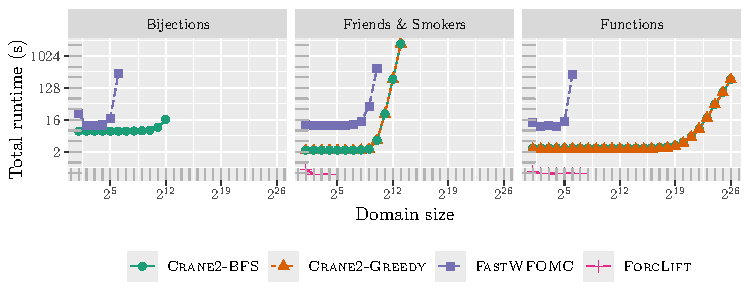
\includegraphics{plot.pdf}
  \caption{The runtime of the algorithms as a function of the domain size. Note
    that both axes are on a logarithmic scale.}\label{fig:plot}
\end{figure*}

\Cref{fig:plot} presents a summary of the experimental results. Only
\textsc{FastWFOMC} and \Cranebfs{} could handle the bijection-counting problem.
For this benchmark, the largest domain sizes these algorithms could accommodate
were \num{64} and \num{4096}, respectively. On the other two benchmarks,
\textsc{ForcLift} had the lowest runtime. However, since it can only handle
model counts smaller than $2^{31}$, it only scales up to domain sizes of
\num{16} and \num{128} for \friends{} and \functions{}, respectively.
\textsc{FastWFOMC} outperformed \textsc{ForcLift} in the case of \friends{}, but
not \functions{}, as it could handle domains of size \num{1024} and \num{64},
respectively. Furthermore, both \Cranebfs{} and \Cranegreedy{} performed
similarly on both benchmarks. Similarly to the \bijections{} benchmark,
\Cranetwo{} significantly outperformed the other two algorithms, scaling up to
domains of size \num{8192} and \num{67108864}, respectively.

One might notice that the runtime of \textsc{FastWFOMC} and \textsc{ForcLift} is
slightly higher on the smallest domain size. This peculiarity is the consequence
of \emph{just-in-time} (JIT) compilation. As \Cranetwo{} is only run once per
benchmark, the JIT compilation time is included in its overall runtime across
all domain sizes. Additionally, while \textsc{ForcLift}'s compilation is
generally faster than that of \Cranetwo{}, neither significantly affects overall
runtime. Specifically, \textsc{ForcLift} compilation typically takes around
\SI{0.5}{\second}, while \Cranetwo{} compilation takes around \SI{2.3}{\second}.

Based on our experiments, which algorithm should be used in practice? If the
sentence can be handled by \textsc{ForcLift} and the domain sizes are reasonably
small, \textsc{ForcLift} is likely the fastest algorithm. In other situations,
\Cranetwo{} is expected to be significantly more efficient than
\textsc{FastWFOMC} regardless of domain size, provided both algorithms can
handle the sentence.

\section{Conclusion and Future Work}\label{sec:conclusion}

In this work, we have presented a scalable automated FOKC-based approach to
FOMC\@. Our algorithm involves completing the definitions of recursive functions
and subsequently translating all function definitions into C++ code. Empirical
results demonstrate that \Cranetwo{} can scale to larger domain sizes than
\textsc{FastWFOMC} while supporting a wider range of sentences than
\textsc{ForcLift}. The ability to efficiently handle large domain sizes is
particularly crucial in the weighted setting, as illustrated by the \friends{}
example discussed in \cref{sec:experiments}, where the model captures complex
social networks with probabilistic relationships. Without this scalability, the
practical usefulness of these models would be limited.

Future directions for research include conducting a comprehensive experimental
comparison of FOMC algorithms to better understand their comparative performance
across various sentences. The capabilities of \Cranetwo{} could also be
characterised theoretically, e.g., by proving completeness for logic fragments
liftable by other algorithms. Additionally, the efficiency of FOMC algorithms
can be further analysed using fine-grained complexity, which would provide more
detailed insights into the computational demands of different sentences.

\todo[inline]{Cite a bunch of papers for the liftable fragments.}

\bibliography{paper}

\end{document}
